\chapter{Pesquisa-ação}
\label{pesquisa_acao}
	\section{Descrição da organização}

		A organização a ser tratada neste trabalho refere-se aos grupos de trabalho das disciplinas de Gestão de Projetos 
		e Portfólio (GPP) e Metodologias de Desenvolvimento de Software (MDS).

		A organização trabalha na produção de software com vários projetos, os quais possuem as seguintes características:

		\begin{itemize}
			\item Uso de dados abertos;
			\item Aplicações WEB e aplicativos \textit{mobile};
			\item Equipe composta de dois times:
				\subitem 1 time de desenvolvimento;
				\subitem 1 equipe de gerência;
			\item Equipes pequenas e inexperientes;
			\item Prazo fixo;
		\end{itemize}

		\subsection{Objeto da ação}

		Para a realização da pesquisa-ação será considerado um projeto em andamento da organização que possui as seguintes características:


		\begin{itemize}
			\item Aplicativo \textit{mobile};
			\item Equipe composta de dois times:
				\subitem 1 time de desenvolvimento com 6 pessoas;
				\subitem 1 equipe de gerência com 6 pessoas;
			\item Membros inexperientes na tecnologia.
			\item Uso de metodologia ágil;
			\item Quantidade de \textit{Sprints}: 7;
			\item Tamanho da \textit{Sprint}: 1 semana;
			\item Dedicação parcial do time, visto que trata-se de uma disciplina.
		\end{itemize}

	\pagebreak


\section{Diagnóstico}
	
	O diagnóstico realizado para ver a situação atual do projeto selecionado para o estudo consistiu na análise 
	dos gráficos de \textit{Burndown} das quatro primeiras \textit{Sprints} e na aplicação de um questionário para o 
	time de desenvolvimento.
	
	\subsection{Análise dos gráficos de \textit{Burndown}}

	Para as quatro primeiras \textit{Sprints} é possível ver nas Figuras \ref{fig:burndown0}, \ref{fig:burndown1}, \ref{fig:burndown2}
	\ref{fig:burndown3} que os pontos realizados não correspondem a pontuação total planejada para a \textit{Sprint}. 
	Assim é possível ver que que nem todas as histórias alocadas foram entregues, o que significa que houve atrasos nas entregas.

	O acompanhamento do \textit{Burndown} por \textit{Sprint} auxiliou na visualização da distribuição do trabalho dentro da \textit{Sprint}.
	Assim foi possível ver, por exemplo, que nas \textit{Sprints} 0 e 1 o time demorou para começar a trabalhar, o que pode ter sido uma causa do atraso. Dessa forma, impactando nas \textit{Sprints} seguintes.

	\begin{figure}[!h]
	\begin{minipage}[b]{0.5\linewidth} 
	\centering
	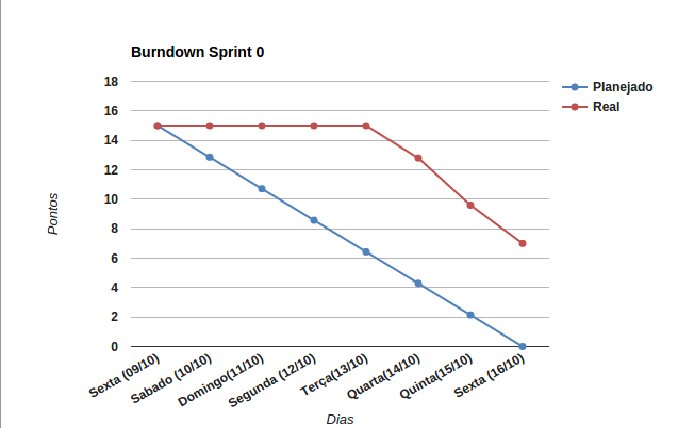
\includegraphics[scale=0.5]{figuras/burndown_sprint0.png}
	\caption{Burndown da Sprint 0.}
	\label{fig:burndown0}
	\end{minipage}
	\hspace{0.5cm} 
	\begin{minipage}[b]{0.5\linewidth}
	\centering
	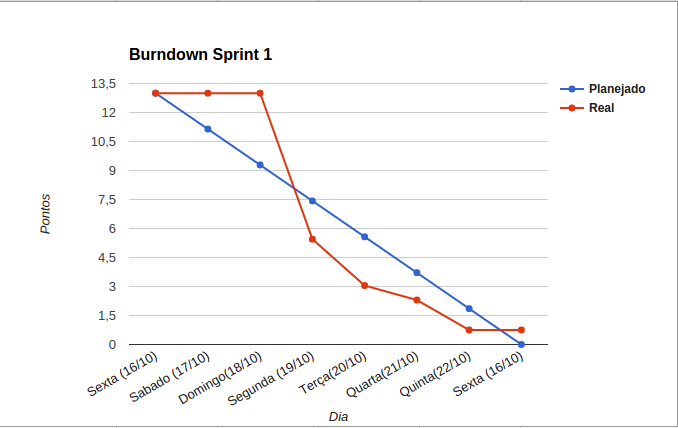
\includegraphics[scale=0.5]{figuras/burndown_sprint1.png}
	\caption{Burndown da Sprint 1.}
	\label{fig:burndown1}
	\end{minipage}
	\end{figure}
	
	\begin{figure}[!h]
	\begin{minipage}[b]{0.5\linewidth} 
	\centering
	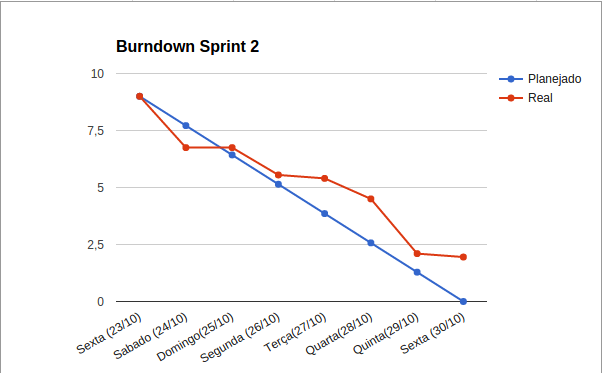
\includegraphics[scale=0.5]{figuras/burndown_sprint2.png}
	\caption{Burndown da Sprint 2.}
	\label{fig:burndown2}
	\end{minipage}
	\hspace{0.5cm} 
	\begin{minipage}[b]{0.5\linewidth}
	\centering
	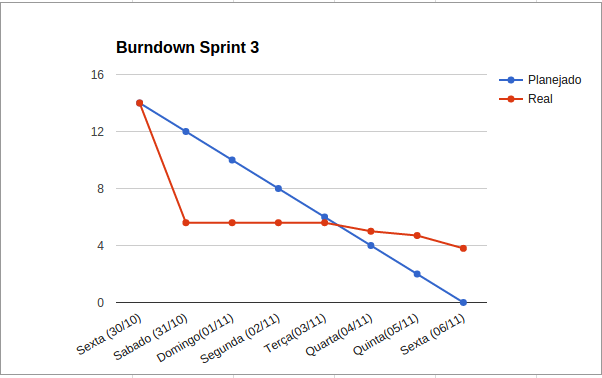
\includegraphics[scale=0.5]{figuras/burndown_sprint3.png}
	\caption{Burndown da Sprint 3.}
	\label{fig:burndown3}
	\end{minipage}
	\end{figure}
	
	\pagebreak

	\subsection{Questionário}

	A fim de coletar dados sobre a percepção dos membros sobre possíveis aspectos que afetaram a entrega nos prazos foi aplicado
	um questionário ao time de desenvolvimento que se encontra no apêndice \ref{apendice:questionario}.



\section{Planejamento da ação}
\section{Execução da ação}
\section{Avaliação da ação}